\chapter{Continuity}

For each of the following, determine whether the function graphed below is continuous at that value. If not, explain why.	\newline\\

\begin{center}
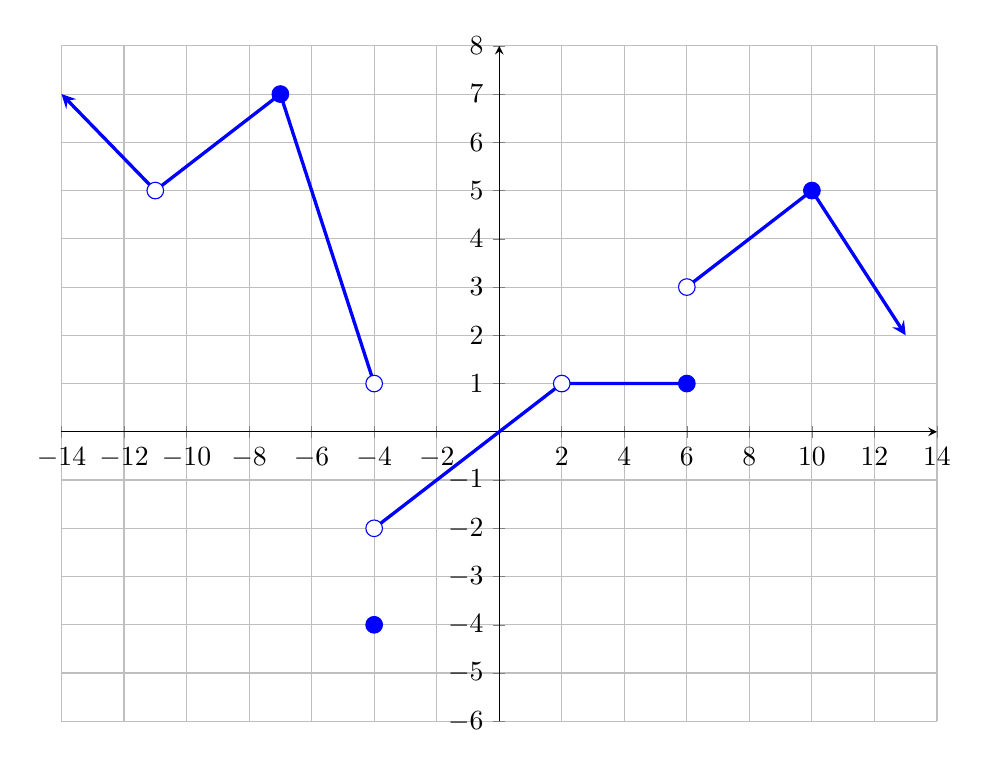
\begin{tikzpicture}[>=stealth]
\begin{axis}
[axis lines = middle, xmin = -14, xmax = 14, xtick = {-14, -12, ..., 14}, ymin = -6, ymax = 8, ytick distance = 1, grid = both, width = 5in, height = 4in]
\draw [->, very thick, blue] (axis cs: -11,5) -- (axis cs: -14,7);
\draw [very thick, blue] (axis cs: -11,5) -- (axis cs: -7,7) -- (axis cs: -4,1);
\draw [very thick, blue] (axis cs: -4,-2) -- (axis cs: 2,1) -- (axis cs: 6,1);
\draw [very thick, blue] (axis cs: 6,3) -- (axis cs: 10,5);
\draw [->, very thick, blue] (axis cs: 10,5) -- (axis cs: 13,2);
\addplot [blue, fill=white, mark=*, only marks, mark size = 3] coordinates {(-11,5) (-4,1) (-4,-2) (2,1) (6,3)};
\addplot [blue, fill=blue, mark=*, only marks, mark size = 3] coordinates {(-7,7) (-4,-4) (6,1) (10,5)};
\end{axis}
\end{tikzpicture}
\end{center}

\begin{multicols}{6}
\begin{enumerate}
	\item $x = -11$
	\item $x = -7$
	\item $x = -4$
	\item $x = 2$
	\item $x = 6$ 
	\item $x = 10$
\end{enumerate}	\setcounter{Review}{\value{enumi}}
\end{multicols}

Identify all discontinuities for each of the following.
\begin{multicols}{2}
\begin{enumerate}		\setcounter{enumi}{\value{Review}}
	\item $f(x) = \frac{x^2-6x}{x^2+6x}$
	\item $f(x) = \frac{x+3}{x-3}$
\end{enumerate}	\setcounter{Review}{\value{enumi}}
\end{multicols}
\begin{multicols}{2}
\begin{enumerate}	\setcounter{enumi}{\value{Review}}
	\item $f(x) = \frac{x+4}{3\ln(x)}$
	\item $f(x) = \frac{2x+5}{x^2-9}$
\end{enumerate}	\setcounter{Review}{\value{enumi}}
\end{multicols}
\begin{multicols}{2}
\begin{enumerate}	\setcounter{enumi}{\value{Review}}
	\item $f(x) = \begin{cases} 
			2 \sin(x), & x < 0 \\
			0, & x = 0 \\
			3x-2, & x > 0	\end{cases}$
	\item $f(x) = \begin{cases}
	e^x - 1, & x \leq 0 \\
	x^2, & x > 0 \end{cases}$
\end{enumerate}	\setcounter{Review}{\value{enumi}}
\end{multicols}
\begin{multicols}{2}
\begin{enumerate}	\setcounter{enumi}{\value{Review}}
	\item $f(x) = \begin{cases}
		\frac{x^2-1}{x+1}, & x < -1 \\
		2x, & x > -1 \end{cases}$
	\item $f(x) = \begin{cases}
		\frac{x^2-1}{x+1}, & x < -1 \\
		2x, & x \geq -1 \end{cases}$
\end{enumerate}
\end{multicols}

\newpage

\section{Answer Key}

\begin{enumerate}
	\item Discontinuous; Not defined at $x = -11$
	\item Continuous
	\item Discontinuous; Left- and right-hand limits are not equal, nor do they equal the function value at $x = -4$
	\item Discontinuous; Not defined at $x = 2$
	\item Discontinuous; Left- and right-hand limits are not equal
	\item Continuous
	\item Discontinuous at $x = 0, -6$
	\item Discontinuous at $x = 3$
	\item Discontinuous at $x = 1$
	\item Discontinuous at $x = \pm 3$
	\item Discontinuous at $x = 0$
	\item Continuous for all values of $x$
	\item Discontinuous at $x = -1$
	\item Continuous for all values of $x$
\end{enumerate}